% =============================================================================
%  Irradiation Studies and Design Optimization of the ATLAS Tile Calorimeter
%  for the High-Luminosity LHC
%
%  Author:  Róbert Astaloš, on behalf of the ATLAS Tile Calorimeter System
%  Style:   tikzposter, A0 portrait, ATLAS colour scheme
%           (reuses the machinery of template/tile_calibration_poster.tex)
%
%  Figures (build/assets/):
%    fig_minidrawer_blockdiagram.png  Valdes 2023 JINST, Fig.1
%    fig_db6_blockdiagram.png         Valdes 2023 JINST, Fig.2
%    fig_db6_tid_test.png             Valdes 2023 JINST, Fig.3
%    fig_mosfet_threshold.png         Valdes 2023 JINST, Fig.4
%    fig_radiation_criteria.pdf       Moayedi TWEPP2025 (ATL-TILECAL-SLIDE-2025-552)
%    fig_lvps_brick.pdf               Moayedi TWEPP2025
%    fig_wire_reduction.pdf           Moayedi TWEPP2025
%    fig_lvps_tests_overview.pdf      Moayedi TWEPP2025
%  Logo (build/logos/): atlas.pdf
%
%  Compile:  pdflatex irradiation_poster.tex   (run twice for references)
% =============================================================================

\documentclass[a0paper,portrait, blockverticalspace=2em, colspace=2em]{tikzposter}
\tikzposterlatexaffectionproofoff
\usepackage{graphicx}
\usepackage{amsmath}
\usepackage{amssymb}
\usepackage{hyperref}
\usepackage{multicol}
\usetikzlibrary{calc}

% Define ATLAS color scheme
\definecolor{maincolor}{HTML}{9e2b2f}
\definecolor{secondarycolor}{RGB}{158, 43, 47}
\definecolor{lightred}{RGB}{237, 199, 201}

% Special colors for radiation-effect callouts
\definecolor{tid}{RGB}{254,128,2}
\definecolor{niel}{RGB}{0,140,0}
\definecolor{see}{RGB}{190,0,62}
\definecolor{sel}{RGB}{0,90,170}
\definecolor{turquoise}{RGB}{0,170,170}

% Set tikzposter theme
\usetheme{Default}

% Override default colors with ATLAS colors
\definecolorstyle{atlascolors}{
    \colorlet{backgroundcolor}{white}
    \colorlet{titlefgcolor}{white}
    \colorlet{titlebgcolor}{maincolor}
    \colorlet{blocktitlefgcolor}{white}
    \colorlet{blocktitlebgcolor}{maincolor}
    \colorlet{blockbodyfgcolor}{black}
    \colorlet{blockbodybgcolor}{lightred!25}
}{
}
\usecolorstyle{atlascolors}

% Custom title style (rounded box, matching the reference template)
\definetitlestyle{sampletitle}{width=760mm, roundedcorners=20, linewidth=2pt, innersep=10pt,
titletotopverticalspace=6mm, titletoblockverticalspace=8mm}{\begin{scope}[line width=\titlelinewidth, rounded corners=\titleroundedcorners] \draw[color=blocktitlebgcolor, fill=titlebgcolor](\titleposleft,\titleposbottom) rectangle (\titleposright,\titlepostop);
\end{scope}
\node[anchor=east, fill=white, rounded corners=10pt, inner sep=10pt, xshift=-22mm]
  at ($(\titleposright,\titlepostop)!0.5!(\titleposright,\titleposbottom)$)
  {
\includegraphics[height=8.6cm]{logos/atlas_transparent.png}};}
\usetitlestyle{sampletitle}

% Title settings
\title{\parbox{0.74\linewidth}{\centering\huge Irradiation Studies and Design
Optimization of the\\[2mm] ATLAS Tile Calorimeter for the High-Luminosity LHC}}
\author{Róbert Astaloš \quad on behalf of the ATLAS Tile Calorimeter System}
\institute{Comenius University Bratislava}
\date{}

\setlength{\columnsep}{0.5cm}

\begin{document}

\maketitle


\begin{columns}

% =========================================================================
%  COLUMN 1 — Context, read-out chain, radiation requirements (shared)
% =========================================================================
\column{0.333}

\block{The ATLAS Tile Calorimeter \& the HL-LHC Upgrade}{
    \begin{itemize}\setlength{\itemsep}{0.3em}
        \item TileCal is the central hadronic sampling calorimeter of ATLAS
        (steel absorber + plastic scintillating tiles, $|\eta|<1.7$). It
        identifies and measures hadronic jets, hadronically decaying
        $\tau$-leptons and missing transverse energy, and assists in muon
        identification.
        \item For the \textbf{High-Luminosity LHC} the instantaneous luminosity
        and pile-up rise steeply. The on-detector electronics are \textbf{fully
        replaced} to provide continuous digital read-out of all channels at
        \textbf{40\,MHz} with improved timing and energy resolution.
        \item The new electronics must survive a much harsher radiation field, so
        every component is qualified against
        \textbf{\textcolor{tid}{Total Ionizing Dose (TID)}},
        \textbf{\textcolor{niel}{Non-Ionizing Energy Loss (NIEL)}} and
        \textbf{\textcolor{see}{Single Event Effects (SEE/SEL)}}.
    \end{itemize}
    \vspace{0.12cm}
    \begin{center}
        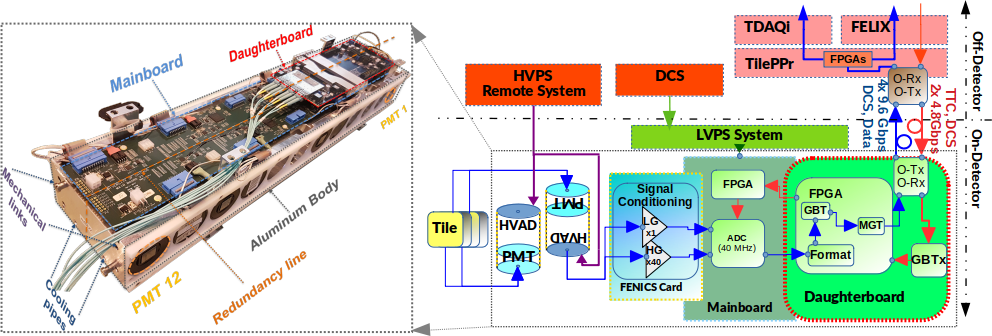
\includegraphics[width=0.98\linewidth]{assets/fig_minidrawer_blockdiagram.png}
    \end{center}
    \vspace{-0.2cm}
    {\small TileCal Phase-II Minidrawer (left) and the on-/off-detector read-out
    chain (right).}
}

\block{Read-Out Chain \& Radiation Requirements}{
    \begin{itemize}\setlength{\itemsep}{0.3em}
        \item The on-detector is segmented into \textbf{896 Minidrawers (MDs)},
        each sampling up to 12 PMTs at 40\,MHz. A MD hosts Front-End Boards
        (shaping), a \textbf{Mainboard (MB)} (digitization), a
        \textbf{Daughterboard (DB)} (timing, control and data transmission), all
        powered by the \textbf{Low-Voltage Power Supply (LVPS)}.
        \item Digitized data are sent off-detector over multi-Gbps optical links to
        the Tile PreProcessor (TilePPr) and FELIX.
        \item Requirements are set from ATLAS simulations at the
        \emph{most-irradiated} positions, scaled by safety factors (SF):
        \textbf{1.5} (simulation), \textbf{$\times$3--5} (lot variation / low-dose-rate)
        and \textbf{1.3} (non-monoenergetic beam).
        \item Daughterboard targets (incl. SFs):
        \textbf{\textcolor{tid}{TID $\approx$ 108 Gy}},
        \textbf{\textcolor{niel}{NIEL $\approx 13.16\times10^{12}$ n/cm$^2$}},
        \textbf{\textcolor{see}{SEE $\approx 4.54\times10^{11}$ h/cm$^2$}}.
    \end{itemize}
    \vspace{0.12cm}
    \begin{center}
        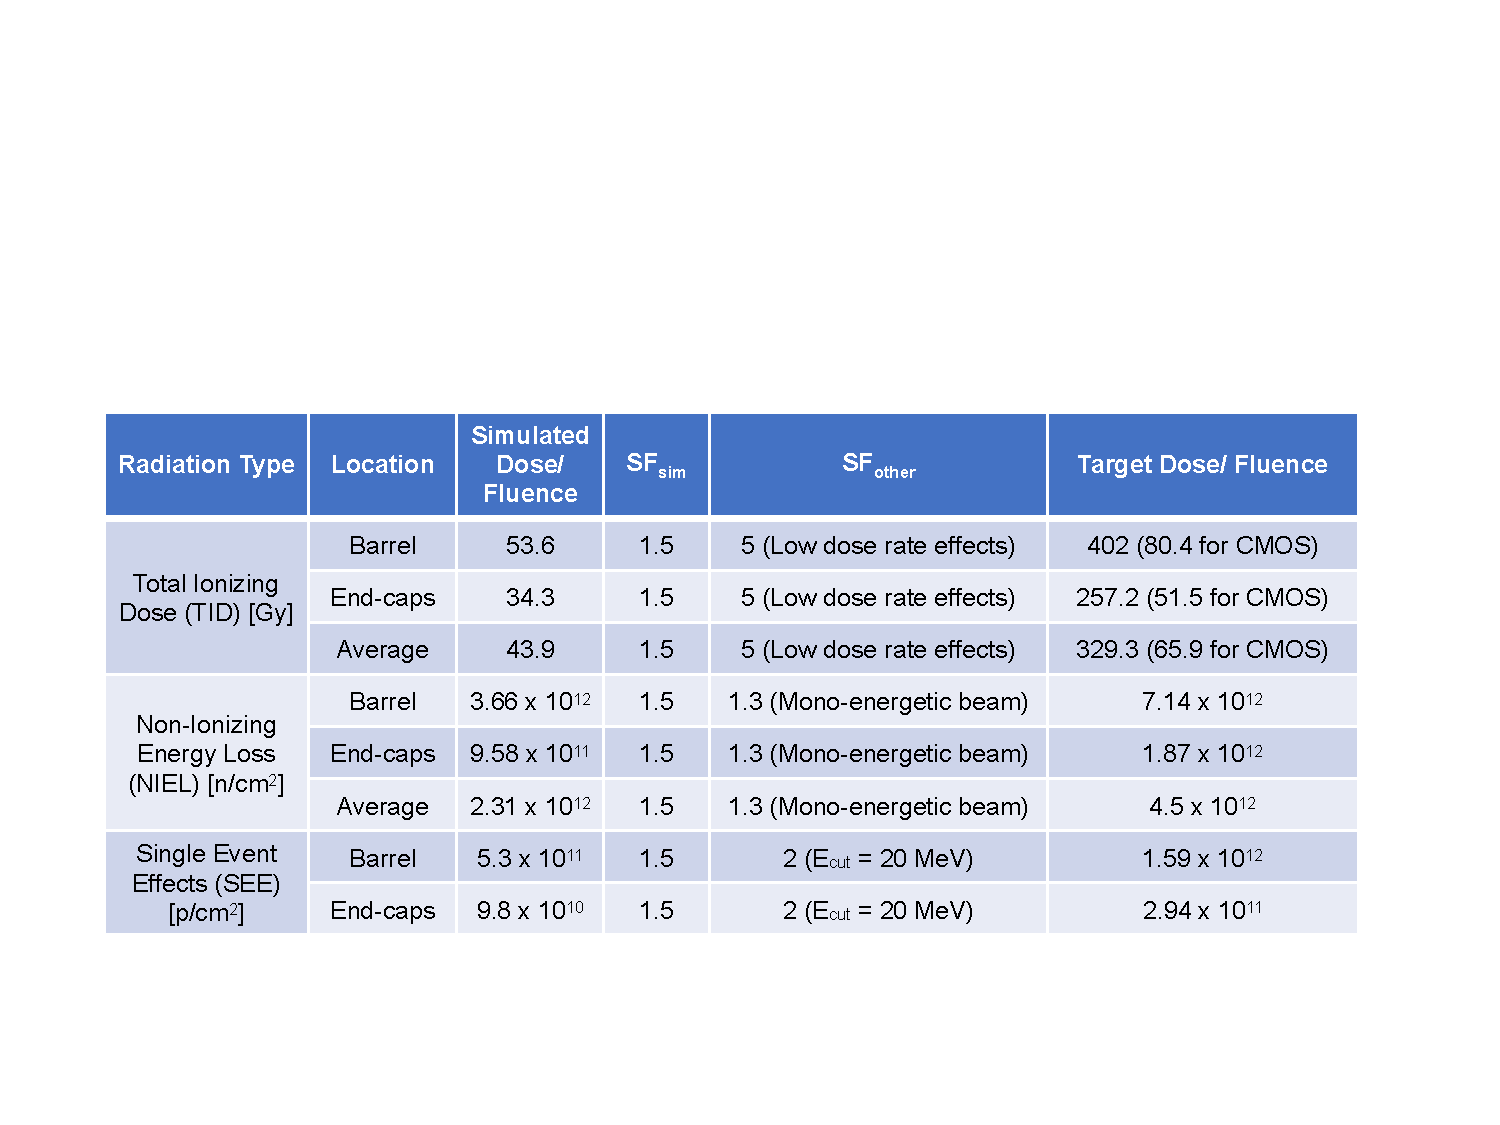
\includegraphics[width=0.99\linewidth]{assets/fig_radiation_criteria.pdf}
    \end{center}
    \vspace{-0.2cm}
    {\small Worked example for the LVPS bricks: simulated dose/fluence scaled by
    safety factors to the qualification target.}
}

\block{References}{
    \small
    \begin{enumerate}\setlength{\itemsep}{0.2em}
        \item ATLAS Collaboration, \emph{Technical Design Report for the Phase-II
        Upgrade of the ATLAS Tile Calorimeter}, CERN-LHCC-2017-019, ATLAS-TDR-028 (2018).
        \item E. Valdes Santurio \textit{et al.}, \emph{Radiation studies performed
        on the High-Luminosity ATLAS TileCal link Daughterboard}, JINST \textbf{18}
        (2023) C04011.
        \item E. Valdes Santurio \textit{et al.}, \emph{Radiation studies on the
        ATLAS Link and Control Daughterboard for the HL-LHC Upgrade}, IEEE NSS MIC
        RTSD (2025).
        \item S. Moayedi (ATLAS), \emph{Upgrade of the ATLAS Tile Calorimeter
        Front-End Power Supply for the HL-LHC}, TWEPP 2025, ATL-TILECAL-SLIDE-2025-552.
    \end{enumerate}
}

% =========================================================================
%  COLUMN 2 — Daughterboard irradiation studies (focus)
% =========================================================================
\column{0.333}

\block{The Link \& Control Daughterboard (DB6)}{
    \begin{itemize}\setlength{\itemsep}{0.15em}
        \item The DB distributes the LHC-synchronized clock, configuration and
        control to the front-end, and continuously transmits the digitized MB
        data off-detector over multi-Gbps optical links.
        \item Now on its sixth revision (\textbf{DB6}), with radiation tolerance
        engineered through a \textbf{double-redundant} scheme: two
        functionally-equivalent halves (A/B), \textbf{Triple Modular Redundancy
        (TMR)}, \textbf{Xilinx Soft Error Mitigation (SEM)}, \textbf{GBT-FEC}
        forward error correction and SEL-protection circuitry.
        \item Key parts: 4$\times$ commercial \textbf{SFP+} (two 4.8\,Gbps
        downlinks, four 9.6\,Gbps uplinks), CERN rad-hard \textbf{GBTx} ASICs,
        Microsemi \textbf{ProASIC3} FPGAs and Xilinx \textbf{Kintex UltraScale
        (KU)} FPGAs. COTS components are used wherever possible.
    \end{itemize}
    \vspace{0.08cm}
    \begin{center}
        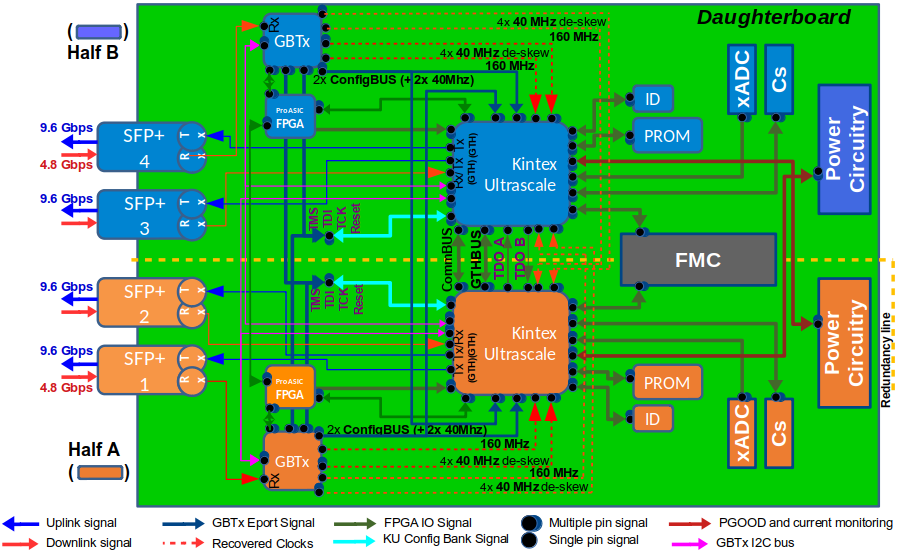
\includegraphics[width=0.60\linewidth]{assets/fig_db6_blockdiagram.png}
    \end{center}
    \vspace{-0.2cm}
    {\small DB6 block diagram: two redundant halves, KU + ProASIC FPGAs, GBTx and
    four SFP+ optical links.}
}

\block{DB6 Radiation Qualification: TID, NIEL \& SEL}{
    \begin{itemize}\setlength{\itemsep}{0.15em}
        \item Four boards (DB6-0\,\dots\,DB6-3) were produced and irradiated separately.
        \item \textbf{\textcolor{tid}{TID}}: DB6-1/-2 $\gamma$-irradiated at the CERN
        CC60 ($^{60}$Co) facility to 220\,Gy (3.37\,Gy/h) and 54\,Gy (0.33\,Gy/h);
        DB6-3 with 54\,MeV protons at IFJ Kraków to $\sim$400\,Gy (2.88\,Gy/h). All
        currents and temperatures stayed stable; no component was damaged by TID.
        \item \textbf{\textcolor{niel}{NIEL}}: DB6-0 and test boards irradiated in the
        TRIGA reactor (JSI Ljubljana) to $14\times10^{12}$ n$_\text{eq}$/cm$^2$. KU
        FPGAs tolerant; ProASIC and FLASH firmware fully recovered after annealing.
        \item \textbf{\textcolor{sel}{SEL}}: 54\,MeV protons to $2.62\times10^{11}$
        p/cm$^2$ and 226\,MeV protons to $1.11\times10^{12}$ p/cm$^2$ —
        \textbf{no single-event latch-ups} observed.
    \end{itemize}
    \vspace{0.08cm}
    \begin{center}
        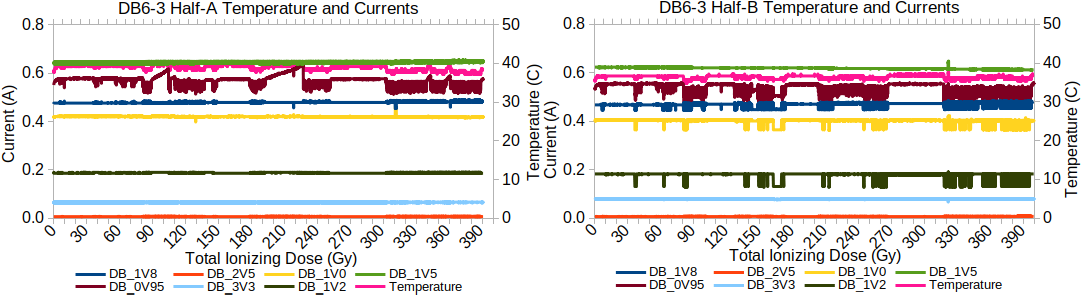
\includegraphics[width=0.56\linewidth]{assets/fig_db6_tid_test.png}
    \end{center}
    \vspace{-0.2cm}
    {\small DB6-3 board currents and FPGA temperature, stable over the full
    $\sim$400\,Gy proton TID run (both halves).}
}

\block{Component Results \& Production}{
    \begin{itemize}\setlength{\itemsep}{0.15em}
        \item \textbf{SFP+}: AVAGO failed and 1/9 CORETEK failed at $9\times10^{12}$
        n/cm$^2$; \textbf{Direktronik 33-4248} and \textbf{FS-Europe SFP-10GSR-85}
        stayed fully functional and were selected.
        \item \textbf{FDFMA3N109 MOSFETs}: threshold shifted with dose $\Rightarrow$
        SEL over-current circuit \textbf{removed}. \textbf{LTC6902} oscillators:
        4/15 failed $\Rightarrow$ \textbf{removed}. INA333, Schottky diodes and
        540BAA oscillators passed.
        \item \textbf{Outcome}: key DB6 components qualified to HL-LHC TID/NIEL/SEL;
        the design is simplified by dropping the radiation-sensitive parts.
        $\sim$\textbf{930 Daughterboards} produced (Stockholm Univ.)\ in \textbf{2026--2027}.
    \end{itemize}
    \vspace{0.08cm}
    \begin{center}
        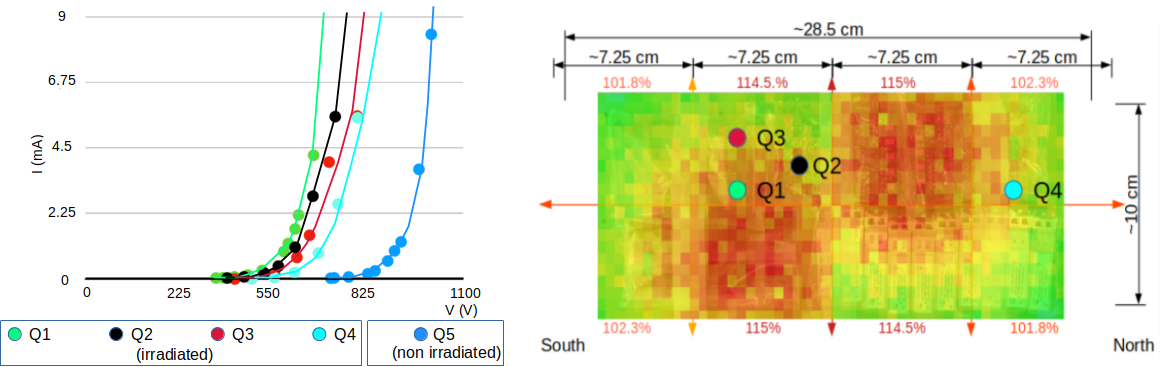
\includegraphics[width=0.46\linewidth]{assets/fig_mosfet_threshold.png}
    \end{center}
    \vspace{-0.2cm}
    {\small FDFMA3N109 threshold shift (IV curves, left) correlated with the reactor
    cavity flux map (right).}
}

% =========================================================================
%  COLUMN 3 — LVPS optimization + conclusions
% =========================================================================
\column{0.333}

\block{LVPS Bricks \& Design Optimization}{
    \begin{itemize}\setlength{\itemsep}{0.3em}
        \item The LVPS sits in the module \emph{finger} — the harshest radiation
        location in TileCal. Phase-2 uses \textbf{8 independent DC-DC ``bricks''}
        per module, each a two-switch forward converter (300\,kHz) stepping
        \textbf{200\,V $\rightarrow$ 10\,V} at $\sim$23\,W. The 8-fold segmentation
        improves reliability and limits the impact of any single failure during
        data-taking.
        \item \textbf{Efficiency}: power MOSFET STB57N65M5 $\rightarrow$
        \textbf{SIHFS9N60A} raised brick efficiency from $\sim$58\% to
        \textbf{$\sim$72\%} (above the $\geq$65\% required by the 77\,kW cooling
        plant) with 65\% smaller gate--source capacitance; the output inductor was
        replaced by a lower-resistance part to cut heating.
        \item \textbf{Control wiring} reduced from \textbf{18} (legacy) to
        \textbf{9} signals (Phase-2 tri-state turn-on / turn-off / keep-state +
        common return), easing the cabling from the service room.
    \end{itemize}
    \vspace{0.25cm}
    \begin{center}
        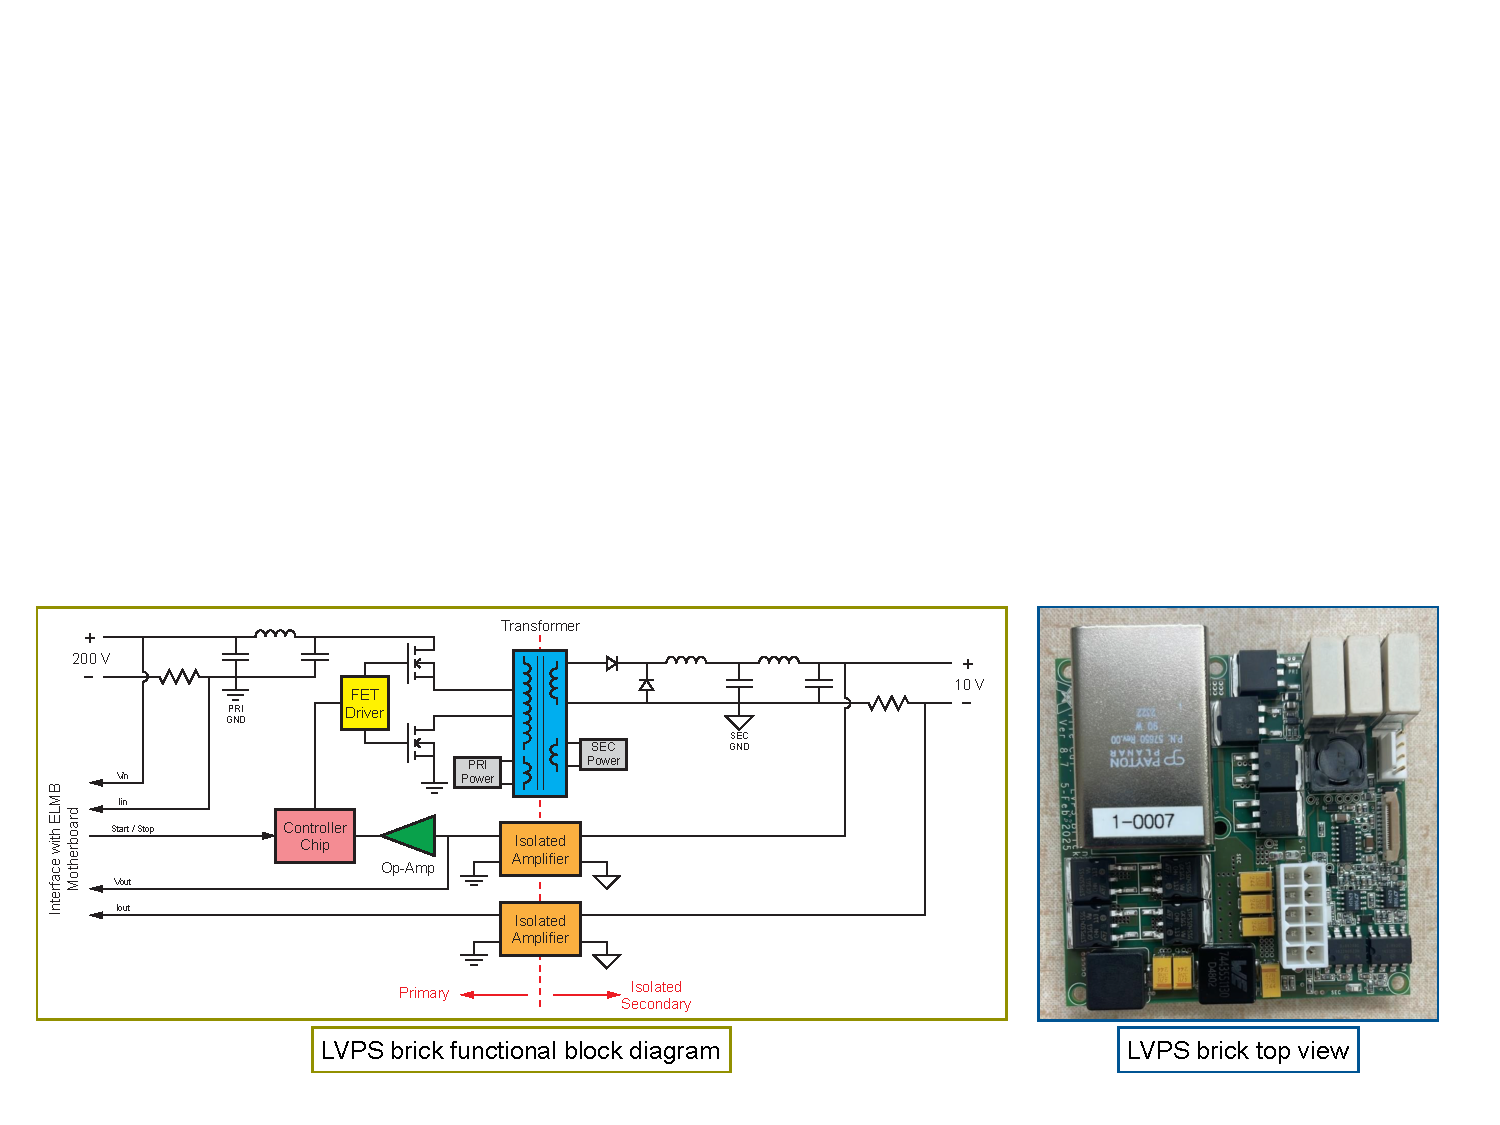
\includegraphics[width=0.99\linewidth]{assets/fig_lvps_brick.pdf}\\[4mm]
        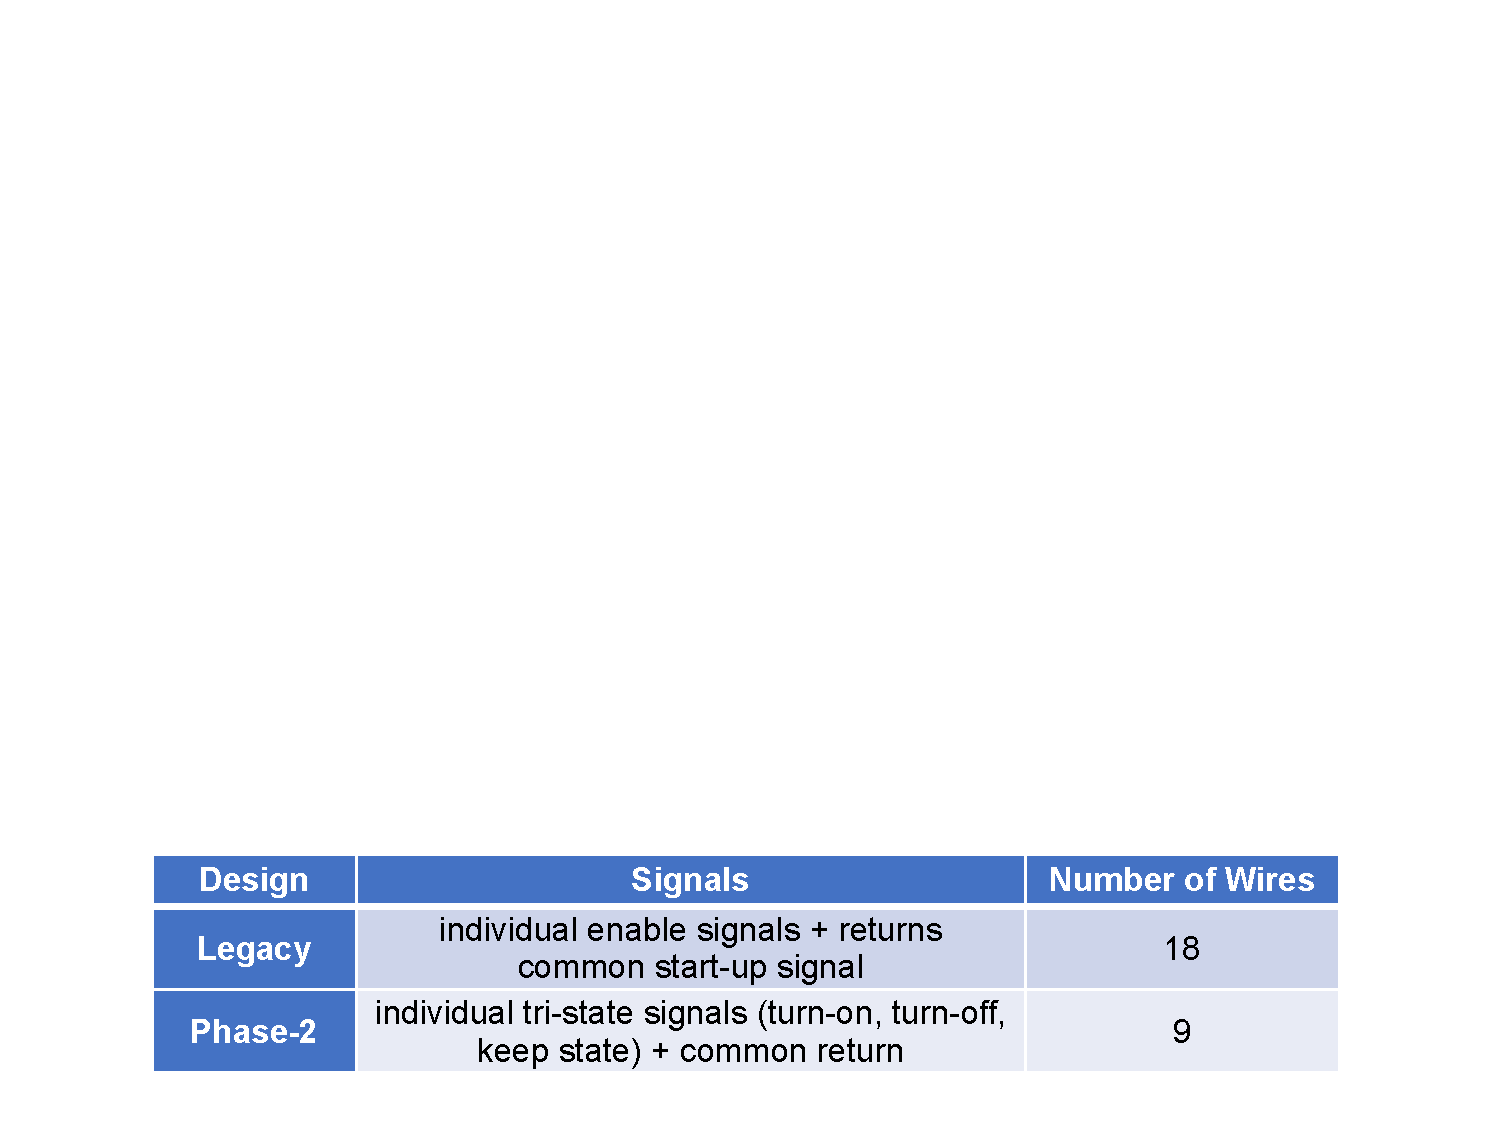
\includegraphics[width=0.78\linewidth]{assets/fig_wire_reduction.pdf}
    \end{center}
    \vspace{-0.2cm}
    {\small LVPS brick functional diagram and top view; legacy vs.\ Phase-2 control
    wiring.}
}

\block{LVPS Radiation Qualification}{
    \begin{itemize}\setlength{\itemsep}{0.3em}
        \item Components qualified for \textbf{\textcolor{tid}{TID}} (CC60; PSI for
        bipolar parts), \textbf{\textcolor{niel}{NIEL}} (TRIGA at JSI, to
        $8\times10^{12}$ n/cm$^2$), \textbf{\textcolor{see}{SEE}} (PIF at PSI,
        200\,MeV protons) and whole-brick \textbf{system-level tests at CERN CHARM}.
        \item Diodes (7 types), \textbf{LT1681} controller, \textbf{LTC6241}
        op-amp, \textbf{LT3080} regulator, \textbf{IR2110} driver and
        \textbf{SIHFS9N60A} MOSFET passed; only small SETs / threshold shifts with
        no impact on brick performance.
        \item \textbf{Isolation amplifier}: SI8920 showed output fluctuations in
        early SEE/TID tests and was temporarily replaced by HCPL7800 for
        pre-production; later tests showed SI8920 is \textbf{stable below 100\,mV
        input}, so the final design constrains its input to $\leq$100\,mV and keeps
        SI8920.
        \item \textbf{CHARM system-level}: pre-production MOSFETs failed at 323\,Gy
        (criterion 80\,Gy) and HCPL7800 at $2.75\times10^{12}$ n/cm$^2$
        (displacement damage) — driving the final component choices.
    \end{itemize}
    \vspace{0.12cm}
    \begin{center}
        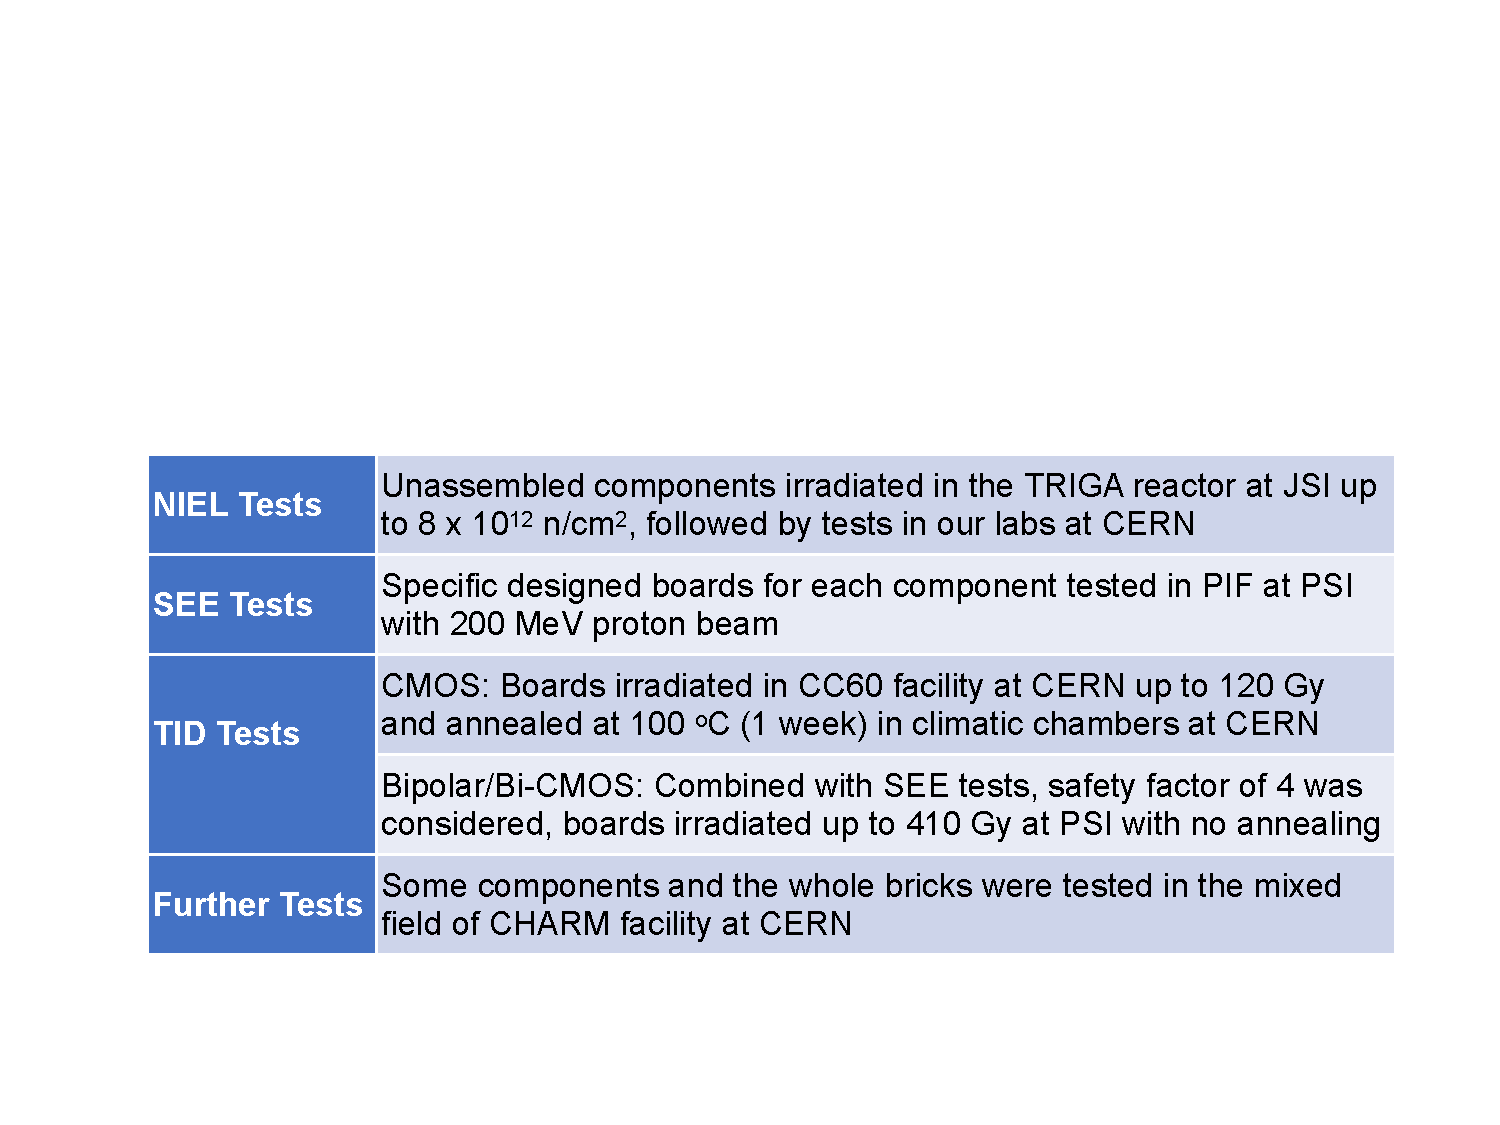
\includegraphics[width=0.99\linewidth]{assets/fig_lvps_tests_overview.pdf}
    \end{center}
    \vspace{-0.2cm}
    {\small Irradiation campaign overview: facility and beam per test type.}
}

\block{Conclusions \& Outlook}{
    \begin{itemize}\setlength{\itemsep}{0.3em}
        \item Both Phase-2 on-detector subsystems — the \textbf{Link Daughterboard}
        and the \textbf{LVPS bricks} — meet the HL-LHC
        \textcolor{tid}{TID}, \textcolor{niel}{NIEL} and \textcolor{see}{SEE}
        requirements after iterative irradiation campaigns.
        \item The irradiation studies \textbf{directly drove design optimization}:
        removal of radiation-sensitive parts on the DB (over-current MOSFETs, QUAD
        oscillators); component selection plus efficiency and wiring improvements on
        the LVPS.
        \item \textbf{Production}: $\sim$930 Daughterboards in 2026--2027; LVPS
        DC-DC converter, ProASIC and KU FPGA lot qualification continuing through
        2025--2026.
    \end{itemize}
}

\end{columns}
\end{document}
